\documentclass{article} 
\usepackage[left=0.75in,top=0.6in,right=0.75in,bottom=0.6in]{geometry} % Document margins
\usepackage{tabularx}
\usepackage{fancyvrb}
%\usepackage[hidelinks]{hyperref}
\usepackage{graphicx}
\usepackage{float}
\usepackage{fancyhdr}
\usepackage{geometry}
\usepackage{lastpage}
\usepackage{tabu}

\geometry{
  top=1in,            % <-- you want to adjust this
  inner=0.5in,
  outer=0.5in,
  bottom=1in,
  headheight=5ex,       % <-- and this
  headsep=4ex,          % <-- and this
}

\pagestyle{fancy}
\fancyhf{}
\rhead{\Large\textit{Old Dominion University}}
\lhead{\Large\textit{ECE 432: Assignment 3}}
\cfoot{Page \thepage \hspace{1pt} of \pageref{LastPage}}
\renewcommand{\footrulewidth}{1pt}

\begin{document}

%----------------------------------------------------------------------------------------
%		 TITLE PAGE
%----------------------------------------------------------------------------------------

\begin{titlepage}

\vspace*{45 pt}
\begin{center}
\Huge{\bf CS 432/532:  Web Science}\\
\huge{Spring 2017\\}

\vspace{60 pt}
\Huge\underline {Assignment 3}\\

\vspace{10 pt}
\Huge{Michael Micros}\\\

\vspace{200 pt}
{\huge \bf {Honor Pledge}}\\
\Large{I pledge to support the Honor System of Old Dominion University. I will refrain from any form of academic dishonesty or deception, such as cheating or plagIiarism. I am aware that as a member of the academic community it is my responsibility to turn in all suspected violations of the Honor Code. I will report to a hearing if summoned. }\\
\vspace {.5cm}

{Signed \_\_\_\_\_\_\_\_\_\_\_\_\_\_\_\_\_\_\_\_\_\_\_\_\_\_\_\_\_\_\_\_\_\_}\\
\today

\end{center}
\end{titlepage}




%----------------------------------------------------------------------------------------
%		PROBLEM 1
%----------------------------------------------------------------------------------------

\section*{{\underline{\huge {Problem 1:}} Downloading HTML from 1000 unique URIs}}

\large{
All the functions necessary to extract the processed HTML from the 1000 unique links are located in ``part1.py''.  The function ``getProcessedHTML'' takes as a parameter the filename of the 1000 URIs, and in turn calls ``getHTML()'' and ``getText()' ' on each URI read from file. All the files are then saved to ``Raw'' and ``Processed''  located in the Part1 directory of the assignment on github.\\

\par The ``getHTML()''  function makes an http request using urllib making sure the response code ia 200 and then returns the raw HTML collected using urlopen().read()\\

\par  The ``getText()''  function makes use of BeautifulSoup to extract the readable text from the HTML, following the example of Tugrur Ates ( http://stackoverflow.com/questions/1936466/beautifulsoup-grab-visible-webpage-text) 

\begin{figure}[H]
 \centering
 	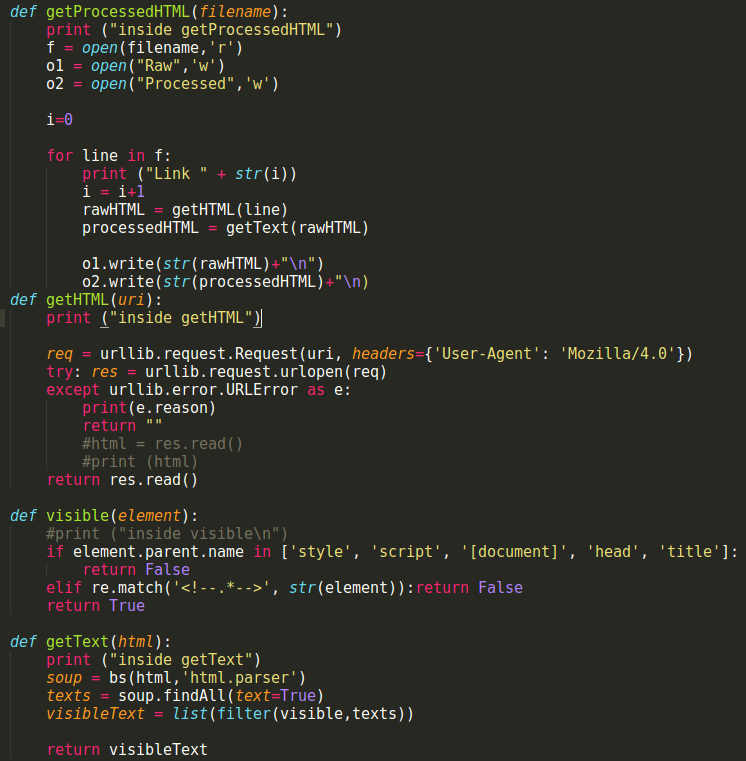
\includegraphics[height=15 cm]{part1.png}
  \caption{Functions that extract 1000 unique links}
\end{figure}


%----------------------------------------------------------------------------------------
%		PROBLEM 2
%----------------------------------------------------------------------------------------

\section*{{\underline{\huge {Problem 2:}} Computation of TFIDF of 10 URIs}}
The query term selected was ``Syria'' and 27 documents had a match. The 10 documents with the highest TFIDF were selected. The processed HTML for each of the 100 URIs was read from file and checked whether it contained the ``term'' which was selected. In the function below, for the documents matching the query term, the number of instances of the term is calculated along with the total number of words the document contains. The the ``write''  function is called, which does additional calculations to compute the TF, IDF and TFIDF. Finally, Bing was the search engine used to calculate the IDF value. \\ 

\begin{figure}[H]
 \centering
 	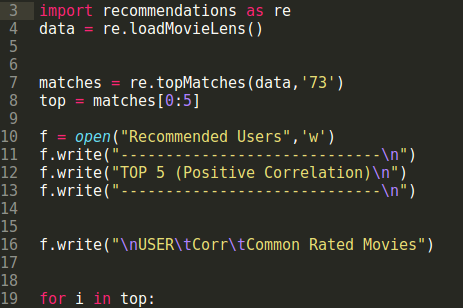
\includegraphics[width = 17 cm]{p2.png}
  \caption{part2.py}
\end{figure}

\begin{tabular}{ |p{2cm}||p{2cm}|p{2cm}|p{2cm}| p{2cm}|p{6cm}| }
 \hline
 TFIDF& Instances &Total words & TF & TFIDF & URI \\
 \hline
 0.2671   & 21    &1063    &0.0198	&  13.5222 &  {http://www.cnn.com/2016/10/09 /politics/trump-pence-syria-disagreement/index.html}    \\
\hline
 0.1290   & 14    & 1468   &0.0095	& 13.5222 &   { http://www.tmimag.com/all-articles/kurdish-people-not-monolith/ }	\\
\hline

 0.0361   & 7      & 2623   &0.0027	&13.5222 	&  {  https://www.newsdeeply.com /refugees/articles/2017/02/14/it-is-scary-to-see-how-the-world-can-change-in-one-night  }  \\
\hline


 0.0270   & 4 	    & 2004   &0.0020	&13.5222	 &    { http://www.nbcnews.com/video /watch-live-actor-ashton-kutcher-testifies-at-hearing-on-ending-modern-slavery-877767747903?cid =sm\_npd  }  \\
\hline


 0.0198   &   3    & 2045   &0.0015	&13.5222	&   { http://www.ncr-iran.org/en/news/iran-world/22008-this-is-the-time-to-confront-iran-regime   }  \\
\hline

0.0155   & 2     & 1742    &0.0011	&13.5222	&       http://www.reuters.com /article/us-usa-trump-russia-ukraine-idUSKBN15U0U0   \\
\hline

 
0.0119   & 1     & 1137    &0.0009	&13.5222	&        http://www.iranfocus.com/en /index.php?option=com \_content\&view=article\&id= 31248\&catid=4\&Itemid=109  \\
\hline

 0.0108   & 1     & 1247    &0.0008	&13.5222	&        http://cnnphilippines.com/world /2017/02/15/us-special-ops-isis-fighters-killed.html   \\
\hline

 0.0106   & 4     & 5096    &0.0008	&13.5222	&         https://themoscowtimes.com /articles/russias-alleged-inf-violation-isnt-so-clear-cut-57161 \\
\hline

 0.0089   & 2     & 3026    &0.0007	&13.5222	&        http://www.newyorker.com/news /john-cassidy/its-time-for-a-proper-investigation-of-trumps-russia-ties  \\
\hline



 \hline
\end{tabular}
\newpage

%----------------------------------------------------------------------------------------
%		PROBLEM 3
%----------------------------------------------------------------------------------------

\section*{{\underline{\huge {Problem 3:}} Ranking the pages}}
The tool use to get the pagerank for the 10 URIs was ``http://pr.eyedomain.com/''. As can be seen in the previous table, there were not that many instances of the query term, with the exception of the first 3 URIs. That probably means that the term "Syria" was present in a title to a link to another page of a large website. That explains why URIs corresponding to ``nbcnews.com'' or ``reuters.com'' find their way to the top of the PageRank table below. \\

\begin{tabular}{ |p{4cm}|p{13cm}|}
 \hline
PageRank & URI \\
0.9		&	http://www.cnn.com\\
\hline
0.8		&	 { http://www.nbcnews.com/video/watch-live-actor-ashton-kutcher-testifies-at-hearing-on-ending-modern-slavery-877767747903?cid=sm\_npd  }  \\
\hline
0.8		&	http://www.reuters.com/article/us-usa-trump-russia-ukraine-idUSKBN15U0U0 \\
\hline
0.8		&	http://www.newyorker.com/news/john-cassidy/its-time-for-a-proper-investigation-of-trumps-russia-ties \\ 
\hline
0.5		&	http://www.ncr-iran.org/en/news/iran-world/22008-this-is-the-time-to-confront-iran-regime \\ 
\hline
0.5		&	http://www.iranfocus.com/en /index.php?option=com \_content\&view=article\&id= 31248\&catid=4\&Itemid=109  \\
\hline
0.4		&	https://www.newsdeeply.com/refugees/articles/2017/02/14/it-is-scary-to-see-how-the-world-can-change-in-one-night \\
\hline
0.0		&	http://www.tmimag.com/all-articles/kurdish-people-not-monolith/ \\
\hline
0.0		&	http://cnnphilippines.com/world/2017/02/15/us-special-ops-isis-fighters-killed.html \\ 
\hline
0.0		&	https://themoscowtimes.com/articles/russias-alleged-inf-violation-isnt-so-clear-cut- \\
\hline

\hline
\end{tabular}


%----------------------------------------------------------------------------------------
\end{document}
